\chapter{Atmospheric Large Eddy Simulation} \label{chap:les}
This chapter focuses on the science of computational fluid dynamics. First, a general description of turbulent flows is given. Second, different techniques for performing computer simulations of turbulent flows are explained and discussed in the context of numerical weather and climate modeling. Finally, the subject model of this thesis, the \acrfull{dales} model, will be discussed in more detail.

\section{Turbulent flows}
Under the right conditions, a fluid (or gas) in motion exhibits circular patterns that vary in size. A flow that features such patterns is described as a \emph{turbulent flow}, and in turbulence theory, the circular patterns are called \emph{eddies} \citep{popeTurbulentFlows2000}. We, as mankind, are surrounded by these kinds of flows in our daily lives. Examples include the flow of water through pipes, airflow around a moving car, waterfalls and the Earth's atmosphere. Because turbulent flows are so predominantly present in our living environment, they are studied intensively by the scientific community and the industry. With these insights, accurate computer models are developed that attempt to predict the effects of turbulence.

To characterize turbulent flows, several scaling laws and non-dimensional numbers have been derived. The \emph{Reynolds number} $\text{Re}$ is defined as the ratio between inertial forces and viscous forces in a fluid: 

\begin{equation}
    \text{Re} = \frac{\text{Inertial forces}}{\text{Viscous forces}} = \frac{u \mathcal{L}}{\nu}
    \label{eq:reynolds_number}
\end{equation}

in which $u$ is the flow speed, $\mathcal{L}$ is a characteristic length scale of the flow, usually determined by the geometry of the flow, and $\nu$ is the kinematic viscosity of the flow. In turbulent flows, the inertial forces dominate and the Reynolds number is therefore high ($>4000$ \citep{popeTurbulentFlows2000}). 

In turbulent flows, the larger an eddy, the more unstable it is. Therefore, large eddies tend to break up into slightly smaller eddies. These smaller eddies are once again unstable and break up into even smaller eddies. This phenomenon is repeated until the eddies are small enough such that the viscous forces in the fluid are able to convert the remaining kinetic energy into heat. The length scale at which the conversion of kinetic energy into heat happens is called the \emph{Kolmogorov length scale}, and is given by:

\begin{equation}
    \eta = \left( \frac{\nu^3}{\varepsilon} \right)^{1/4}
    \label{eq:kolmogorov-length}
\end{equation}

where $\varepsilon$ is the rate of dissipation of kinetic energy.

\section{Turbulence modeling}
The motion of fluids is mathematically described by the famous Navier-Stokes equations, of which various forms exist. Here, the form that applies to \emph{incompressible} fluids is used. An incompressible fluid is a fluid whose density does not change as a result of pressure changes \citep{popeTurbulentFlows2000}. Using Einstein's summation convention, the Navier-Stokes equations for an incompressible fluid are given by:

\begin{align}
    &\frac{\partial u_i}{\partial x_i} = 0, \label{eq:ns_mass_conservation}\\
    &\frac{\partial u_i}{\partial t} + u_j \frac{\partial u_i}{\partial x_j} = - \frac{1}{\rho} \frac{\partial p}{\partial x_i} + \nu \frac{\partial^2 u_i}{\partial x_j^2}+ g_i,
    \label{eq:ns_momentum}
\end{align}

where $u_i$ denotes the velocity ($i=1,2,3$, corresponding to $x$, $y$ and $z$ directions respectively), $\rho$ is the density, $p$ is the pressure, $g_i$ denotes the body forces and $\nu$ is the kinematic viscosity. If one desires to study the evolution of a flow field in time, one would have to find a solution to \Autoref{eq:ns_mass_conservation,eq:ns_momentum}. However, no analytical solution to the general form of these equations has been found. To find an approximate solution to the Navier-Stokes equations, numerical methods are often used. 

The objective of solving \Autoref{eq:ns_mass_conservation, eq:ns_momentum} such that eddies of all scales are represented imposes two requirements on the computational mesh. First, the mesh has to span a large enough area such that the largest scales can be captured. Second, the mesh spacing must be small enough to be able to represent the Kolmogorov scale. If both requirements are met, all turbulent motions can be resolved and no parameterizations are needed. This technique is called \acrfull{dns} \citep{popeTurbulentFlows2000}. While \acrshort{dns} is very accurate, it is computationally \emph{very} expensive. Even for moderate domain sizes, \acrshort{dns} is often unfeasible due to the resolution requirements.

\citet{smagorinskyGeneralCirculationExperiments1963} proposed the idea of explicitly resolving only the largest, most energetic eddies and using a model for the smaller eddies. This idea was further worked out by \citet{lilly1967representation} and \citet{deardorffThreedimensionalNumericalStudy1974}. To arrive at the governing equations of \acrshort{les}, a filter is applied to \Autoref{eq:ns_mass_conservation,eq:ns_momentum}. This filter can be thought of as a low-pass filter; small-scale, high-frequency motions are filtered out and large-scale motions remain \citep{leonardEnergyCascadeLargeEddy1975}. After the filtering operation, the filtered Navier-Stokes equations are obtained:

\begin{align}
    &\frac{\partial \overline{u}_i}{\partial x_i} = 0, \label{eq:continuity_filtered}\\ 
    &\frac{\partial \overline{u}_i}{\partial t} + \frac{\partial \overline{u}_i \overline{u}_j}{\partial x_j} = - \frac{1}{\rho} \frac{\partial \overline{p}}{\partial x_i} + \nu \frac{\partial^2 \overline{u}_i}{\partial x_j^2} + f_i - \frac{\partial \tau_{ij}}{\partial x_j}.  \label{eq:momentum_filtered}
\end{align}

In \Autoref{eq:momentum_filtered}, it can be seen that the term $\partial \tau_{ij} / \partial x_j$ arises, which is called the \emph{subfilter-scale stress tensor}. The evaluation of $\tau_{ij}$ requires a model, called the \emph{subfilter-scale model}. Some examples of subfilter-scale models include the Smagorinsky model \citep{smagorinskyGeneralCirculationExperiments1963}, the Bardina model \citep{bardinaImprovedSubgridscaleModels1980} or the Vreman model \citep{vremanEddyviscositySubgridscaleModel2004}. These models are turbulent viscosity models, which assume that the subfilter-scale motions similarly dissipate kinetic energy as the viscous forces in the fluid. Because the small-scale turbulent motions are modeled in an \acrshort{les}, the required resolution of the computational mesh is significantly lower compared to \acrshort{dns}, making it a suitable technique for a wider variety of problems, specifically problems that require larger domain sizes. Still, a high enough resolution must be used such that enough of the energy-carrying eddies are resolved. For this reason, \acrshort{les} is not considered as computationally cheap.

Instead of attempting to (partly) \emph{resolve} the small-scale turbulent motions, as done with \acrshort{dns} and \acrshort{les}, one could also choose to \emph{model} the effect of turbulence on the mean flow field. Models that follow this line of thought are referred to as \acrlong{rans} models \citep{popeTurbulentFlows2000}. The governing equations of a \acrshort{rans} model follow from applying the Reynolds averaging rules to the Navier-Stokes equations (\Autoref{eq:ns_mass_conservation,eq:ns_momentum}). To this end, the velocity field $u_i$ is decomposed into a mean part $\overline{u_i}$, and a part $u_i^\prime$ that represents fluctuations due to turbulence, such that:

\begin{equation}
    u_i = \overline{u_i} + u_i^\prime.
    \label{eq:reynolds_decomposition}
\end{equation}

This act is called \emph{Reynolds decomposition}. This decomposition operation is applied to \Autoref{eq:ns_mass_conservation,eq:ns_momentum}, yielding:

\begin{align}
    &\frac{\partial \left( \overline{u_i} + u_i^\prime \right)}{\partial x_i} = 0, \label{eq:reynolds_mass}\\
    &\frac{\partial \left( \overline{u_i} + u_i^\prime \right)}{\partial t} + \left( \overline{u_j} + u_j^\prime \right) \frac{\partial \left( \overline{u_i} + u_i^\prime \right)}{\partial x_j} = - \frac{1}{\left( \overline{\rho} + \rho^\prime \right)} \frac{\partial \left( \overline{p} + p^\prime \right)}{\partial x_i} + \nu \frac{\partial^2 \left( \overline{u_i} + u_i^\prime \right)}{\partial x_j^2} + \overline{g_i} + g_i^\prime,
    \label{eq:reynolds_momentum}
\end{align}

Finally, all terms in \Autoref{eq:reynolds_mass,eq:reynolds_momentum} are averaged in time, yielding the \acrshort{rans} equations \citep[Chapter~4]{popeTurbulentFlows2000}:

\begin{align}
    &\frac{\partial \overline{u_i}}{\partial x_i} = 0, \label{eq:rans_mass}\\
    &\frac{\partial \overline{u_i}}{\partial t} + \overline{u_j} \frac{\partial \overline{u_i}}{\partial x_j} = - \frac{1}{\overline{\rho}} \frac{\partial \overline{p}}{\partial x_i} + \nu \frac{\partial^2 \overline{u_i}}{\partial x_j^2} + \overline{g_i} + \frac{\partial \overline{u_i^\prime u_j^\prime}}{\partial x_i}. \label{eq:rans_momentum}
\end{align}

The term $\overline{u_i^\prime u_j^\prime}$ in \Autoref{eq:rans_momentum} is called the Reynolds stress. A \acrshort{rans} model only solves \Autoref{eq:rans_mass,eq:rans_momentum} for the mean quantities $\overline{u_i}$ and $\overline{p}$, meaning that the Reynolds stress term needs to be modeled. Often used models include turbulent viscosity models (similar to \acrshort{les}) or Reynolds stress models, which use transport equations to evaluate the Reynolds stress \citep{popeTurbulentFlows2000}. More recently, the use of machine learning methods has been explored for modeling the Reynolds stress \citep{bruntonMachineLearningFluid2020}. Because turbulence is not explicitly resolved by \acrshort{rans} models, the required resolution is the least out of the three simulation techniques. For this reason, \acrshort{rans} is computationally cheap but is also the least accurate.

A visual comparison between the three techniques can be found in \Autoref{fig:turbulence_model_comparison}. Following the theory, it can be seen that compared to the full-resolved \acrshort{dns} flow field, the \acrshort{les} simulation is able to reproduce most of the large-scale turbulent features. Especially at a greater distance from the entry of the main jet (at the top of the image), \acrshort{les} loses the small-scale details compared to \acrshort{dns}. The \acrshort{rans} flow field shows little instabilities at all as a consequence of the time averaging. 

\begin{figure}
    \centering
    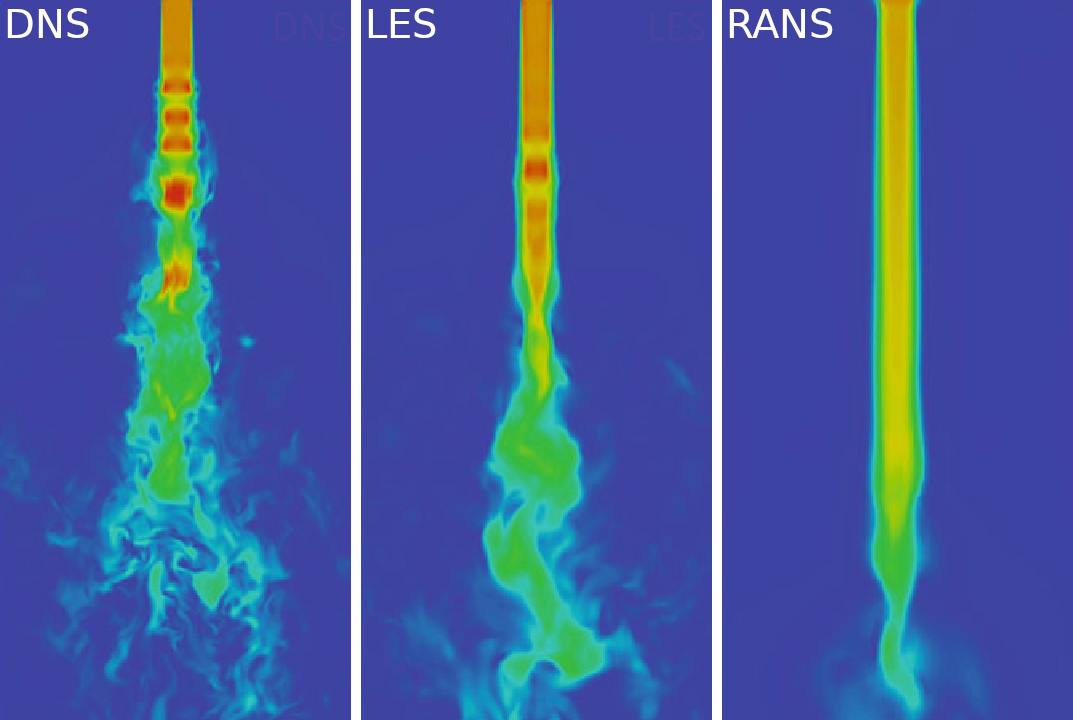
\includegraphics[width=\textwidth]{../images/drawings/turbulence_model_comparison.png}
    \caption{Visualization of the velocity distribution of a jet flow, as simulated by the three turbulence modeling techniques. From left to right: \acrfull{dns}, \acrfull{les} and \acrfull{rans}. Adapted from \citet{Rodriguez2019}.}
    \label{fig:turbulence_model_comparison}
\end{figure}
\section{Towards high-resolution weather and climate models}
Due to limitations of computational capacity, global numerical weather and climate models often use grids with low horizontal resolution in combination with the \acrshort{rans} formulation. Due to the low resolution, small-scale phenomena, such as cloud formation, have to be parameterized, which introduces significant uncertainties in weather forecasts and climate projections \citep{slingoUncertaintyWeatherClimate2011}. At higher resolutions (in the order of 1-2 kilometers), these small-scale processes are still not fully resolved, but their influence on the resolved flow field can be captured partly \citep{scharKilometerScaleClimateModels2020}. Therefore, global weather and climate models are continuously developed and updated to support increasing resolutions. One of the problems that arise at these high resolutions is that the aforementioned parameterizations do not perform well when convective processes are partly resolved, and therefore have to be adapted to this fact \citep{wyngaardNumericalModelingTerra2004}. The range of resolutions at which this problem persists is also referred to as the \emph{terra incognita}, or the \emph{grey zone} \citep{schalkwijkWeatherForecastingUsing2015,wyngaardNumericalModelingTerra2004}. Furthermore, \citet{scharKilometerScaleClimateModels2020} identify the exploitation of modern \acrlong{gpu} technology as another key challenge towards high-resolution weather and climate modeling. \acrshort{gpu} technology will be explained more thoroughly in \Autoref{chap:gpgpu}, but for now it suffices to say that a \acrshort{gpu} is a hardware device that can accelerate specific calculations of a weather or climate model. To allow a numerical weather or climate model to make use of this specialized hardware, significant changes to the source code are needed.

On the other end of the resolution spectrum, the \acrshort{les} technique has been used to develop atmospheric models that explicitly resolve turbulent motions and do not require the aforementioned parameterizations, therefore also lacking the associated uncertainties \citep{schalkwijkWeatherForecastingUsing2015}. Hence, \acrshort{les} can potentially act as a replacement for \acrshort{rans}-based models for high-resolution atmospheric modeling. However, as discussed before, the computational burden associated with \acrshort{les} is quite high, which limits the application of \acrshort{les} over very large domain sizes. Again, \acrshort{gpu}s can help speed up calculations, making large-scale \acrshort{les} possible. The use of \acrshort{gpu}s in \acrshort{les} has been demonstrated by \citet{schalkwijkWeatherForecastingUsing2015}, who were able to do a weather forecast-like simulation over the entire Netherlands using an \acrshort{les} model.

\section{\acrshort{dales}}
The \acrfull{dales} model is a large-eddy simulation model designed for high-resolution modeling of the atmosphere and its processes, like cloud formation and precipitation \citep{heusFormulationDutchAtmospheric2010,ouwerslootLargeEddySimulationComparison2017}. 

\subsection{Prognostic equations}
\acrshort{dales} uses five prognostic variables to define the state of the atmosphere: three velocity components $u$, $v$ and $w$, the liquid water potential temperature $\theta_l$ and the total water specific humidity $q_t$. The general form of the momentum equation (\Autoref{eq:ns_momentum}) for the atmosphere is given by \citep{stullIntroductionBoundaryLayer1988}:

\begin{equation}
    \frac{\partial u_i}{\partial t} + u_j \frac{\partial u_i}{\partial x_j} = - \frac{1}{\rho} \frac{\partial p}{\partial x_i} - g \delta_{i3} + f_i. \label{eq:momentum_atmos}
\end{equation}

Compared to \Autoref{eq:ns_momentum}, \Autoref{eq:momentum_atmos} lacks the viscous term and introduces the gravity $g$. In atmospheric flows, the Reynolds number (\Autoref{eq:reynolds_number}) is large, which is why the viscous term can be safely neglected. \acrshort{dales} makes use of the \emph{anelastic approximation}, meaning that density differences are neglected except for the vertical direction \citep{boingInteractionDeepConvective2014}. To this end, a time-independent base density profile $\rho_0$ is introduced, which only varies in the vertical direction. \Autoref{eq:momentum_atmos} then can be written as:

\begin{equation}
    \frac{\partial u_i}{\partial t} + \frac{1}{\rho_0} \frac{\partial \rho_0 u_i u_j}{\partial x_j} = - \frac{1}{\rho} \frac{\partial p}{\partial x_i} - g \delta_{i3} + f_i. \label{eq:momentum_atmos_rho0}
\end{equation}

The pressure gradient $\partial p / \partial x_i / \rho$ can be expressed as a function of the virtual potential temperature \citep{boingInteractionDeepConvective2014}:

\begin{equation}
    \frac{1}{\rho} \frac{\partial p}{\partial x_i} \approx - g \delta_{i3} - g \delta_{i3} \frac{\theta_v - \theta_{v,e}}{\theta_{v,e}} + \frac{\partial}{\partial x_i} \frac{p^\prime}{\rho_e}, \label{eq:pressure_grad}
\end{equation}

in which the subscript $e$ denotes an environmental state that only varies in the vertical direction and in time. $p^\prime$ is the pressure fluctuation from the environmental pressure $p_e$. In turn, $\theta_v$ can be evaluated from the prognostic variables:

\begin{equation}
    \theta_v = \left( \theta_l + \frac{L_v}{c_{pd} \Pi_e} q_c \right) \left( 1 - \left( 1 - \frac{R_v}{R_d} q_t \right) - \frac{R_v}{R_d} q_c \right), \label{eq:theta_v} 
\end{equation}

where $L_v$, $c_{pd}$, $R_v$ and $R_d$ are constants (their meaning and values are omitted here for brevity but can be found in e.g. \citet{stullIntroductionBoundaryLayer1988}), $\Pi_e = (p_e/p_0)^{R_d/c_{pd}}$ in which $p_0=10^5$ is a reference pressure and $q_c$ is the cloud condensate, which can be diagnosed. After combining \Autoref{eq:momentum_atmos_rho0,eq:pressure_grad} and applying the \acrshort{les} filtering operation, we arrive at the governing momentum equation of \acrshort{dales}:

\begin{align}
    \frac{\partial \overline{u}_i}{\partial t} &= - \frac{1}{\rho_0} \frac{\partial \rho_0 \overline{u}_i \overline{u}_j}{\partial x_j} - \frac{\partial \pi}{\partial x_i} + g \delta_{i3} \frac{\overline{\theta_v} - \theta_{v,e}}{\theta_{v,e}} + f_i - \frac{\partial \tau_{ij}}{\partial x_j} \label{eq:momentum_conservation}
\end{align}

where $\pi$ denotes the modified pressure given by $\pi = p^\prime/\rho_e + 2e/3$, where $e$ is the turbulence kinetic energy. Furthermore, $f_i$ contains the body forces (e.g., the Coriolis force) and $\tau_{ij}$ is the subfilter-scale stress tensor. Similarly, the momentum equation for a scalar $\varphi$, where $\varphi \in \{\theta_l, q_t\}$, is given by:

\begin{equation}
    \frac{\partial \overline{\varphi}}{\partial t} = - \frac{1}{\rho_0} \frac{\partial \rho_0 \overline{u}_j \overline{\varphi}}{\partial x_j} - \frac{\partial R_{u_j,\varphi}}{\partial x_j} + S_\varphi,
\end{equation}

in which $R_{u_j,\varphi}$ is a sub-filter scale flux and $S_\varphi$ is a source term.

\subsection{Subfilter-scale model}
\acrshort{dales} uses an eddy-viscosity model to evaluate the subfilter-scale fluxes. Following this model, the subfilter-scale stress tensor in \autoref{eq:momentum_filtered} is given by:

\begin{equation}
    \tau_{ij} = - K_m \left( \frac{\partial \overline{u}_i}{\partial x_j} + \frac{\partial \overline{u}_j}{\partial x_i} \right),
\end{equation}

in which $K_m$ is the eddy viscosity for momentum. For scalars, the subfilter-scale flux $R_{u_j,\varphi}$ is given by:

\begin{equation}
    R_{u_j,\varphi} = - K_h \frac{\partial \overline{\varphi}}{\partial x_j},
\end{equation}

where $K_h$ is the eddy diffusivity for thermodynamic scalars. $K_m$ and $K_h$ can be calculated in two ways: as a function of the turbulence kinetic energy $e$ as formulated by \citet{deardorffStratocumuluscappedMixedLayers1980} or using the Smagorinsky model. Following \citet{deardorffStratocumuluscappedMixedLayers1980}, $K_m$ and $K_h$ are modeled as:

\begin{equation}
    K_m = c_m \lambda e^{1/2}, \quad K_h = c_h \lambda e^{1/2},
\end{equation}

where $c_m$ and $c_h$ are constants and $\lambda$ is a length scale. This formulation introduces a new prognostic variable, namely the turbulence kinetic energy $e$. The prognostic equation for $e$ is given by:

\begin{equation}
    \frac{\partial e}{\partial t} = - \frac{\partial \overline{u}_j e}{\partial x_j} - \tau_{ij} \frac{\partial \overline{u}_i}{\partial x_j} + \frac{g}{\theta_0} R_{w,\theta_v} - \frac{\partial R_{u_j,e}}{\partial x_j} - \frac{1}{\rho_0} \frac{\partial R_{u_j,\pi}}{\partial x_j} - \varepsilon,
    \label{eq:deardorff_tke}
\end{equation}

of which the first two terms can be calculated from the resolved velocity field. The terms containing subfilter-scale fluxes ($R_{u_j,\varphi}$) and the dissipation rate $\varepsilon$ have to be parameterized. The third term, representing the subfilter-scale production of \acrshort{tke} due to buoyancy effects, is parameterized as:

\begin{equation}
    \frac{g}{\theta_0} R_{w,\theta_v} = \frac{g}{\theta_0} \left( A R_{w,\theta_l} + B R_{w,q_t}\right),
    \label{eq:sfs_buoy}
\end{equation}

in which $A$ and $B$ are coefficients whose value depends on moisture and temperature. Next, the fourth and fifth terms of \Autoref{eq:deardorff_tke}, which represent the turbulent transport of \acrshort{tke}, are combined into a single term:

\begin{equation}
    - \frac{\partial}{\partial x_j} \left( R_{u_j,e} + \frac{1}{\rho_0} R_{u_j,\pi} \right) = \frac{\partial}{\partial x_j} \left( 2 K_m \frac{\partial e}{\partial x_j} \right).
    \label{eq:sfs_turb}
\end{equation}

Finally, the dissipation rate $\varepsilon$ is modeled as:

\begin{equation}
    \varepsilon = \frac{c_{\varepsilon}e^{3/2}}{\lambda}, \quad c_\varepsilon = 0.19 + 0.51 \frac{\lambda}{\Delta},
    \label{eq:sfs_diss}
\end{equation}

where $\Delta$ is the \acrshort{les} filter width. \Autoref{eq:deardorff_tke,eq:sfs_buoy,eq:sfs_turb,eq:sfs_diss} are combined into a prognostic equation for the \emph{square root} of $e$:

\begin{equation}
    \begin{split}
        \frac{\partial e^{1/2}}{\partial t} = &- \overline{u}_j \frac{\partial e^{1/2}}{\partial x_j} + \frac{1}{2e^{1/2}} \left( K_m \left( \frac{\partial \overline{u}_j}{\partial x_i} + \frac{\partial \overline{u}_i}{\partial x_j} \right) \frac{\partial \overline{u}_i}{\partial x_j} - K_h \frac{g}{\theta_0} \frac{\partial}{\partial z} \left( A \overline{\theta}_l + B \overline{q}_t\right) \right) \\ &+ \frac{\partial}{\partial x_j} \left( 2 K_m \frac{\partial e^{1/2}}{\partial x_j}\right) - \frac{c_{\varepsilon} e}{2 \lambda}
    \end{split}
    \end{equation}

\subsection{Mass conservation} \label{sec:dales_poisson}
Following the anelastic approximation, the expression for mass conservation reads:

\begin{equation}
    \frac{\partial \rho_0 \overline{u}_i}{\partial x_i} = 0. \label{eq:mass_conservation}
\end{equation}

\autoref{eq:mass_conservation} states that the divergence of the velocity field $u_i$ must be equal to zero. This condition can be enforced by using Chorin's projection method \citep{chorinNumericalSolutionNavierStokes1967}. Per Chorin's method, the time integration of $\overline{u}_i$ is split into two parts. The first step consists of calculating an intermediate velocity field that is not divergence-free, by evaluating all right-hand terms of \autoref{eq:momentum_conservation}, except for the pressure term:

\begin{equation}
    \frac{\partial \overline{u}^*_i}{\partial t} = - \frac{1}{\rho_0} \frac{\partial \rho_0 \overline{u}_i \overline{u}_j}{\partial x_j} + g \delta_{i3} \frac{\overline{\theta_v} - \theta_{v,e}}{\theta_{v,e}} + f_i - \frac{\partial \tau_{ij}}{\partial x_j}, \label{eq:chorin_step1}
\end{equation}

where $\overline{u}^*_i$ denotes the velocity field that is not divergence-free. From \autoref{eq:chorin_step1}, it follows that:

\begin{equation}
    \frac{\partial \overline{u}_i}{\partial t} = \frac{\partial \overline{u}^*_i}{\partial t} - \frac{\partial \pi}{\partial x_i}. \label{eq:chorin_step2}
\end{equation}

To obtain an explicit equation for the pressure $\pi$, the divergence of \autoref{eq:chorin_step2} can be taken. After rearranging terms, this leads to the following expression:

\begin{equation}
    \frac{\partial^2 \pi}{\partial x_i^2} = \frac{\partial}{\partial x_i} \frac{\partial \overline{u}_i^*}{\partial t}. \label{eq:poisson_equation}
\end{equation}

Despite its simplicity at first sight, \Autoref{eq:poisson_equation} is often the most costly part of a \acrshort{cfd} simulation \citep{costaFFTbasedFinitedifferenceSolver2018}. \acrshort{dales} offers the option to solve this equation with the \acrfull{fft} algorithm, which can offer significantly better performance compared to iterative solvers that are often used \citep{hockneyFastDirectSolution1965}. After \Autoref{eq:poisson_equation} is solved, the velocity field is corrected according to \Autoref{eq:chorin_step2}, which concludes the projection method.

\subsection{Discretization}
For the discretization of the governing equations, \acrshort{dales} makes use of an Arakawa C-grid \citep{arakawaComputationalDesignBasic1977}. This means that the velocity components are defined at the faces of the grid cells, while pressure, turbulence kinetic energy and scalars are defined at the centers of the grid cells. \acrshort{dales} features several numerical schemes to evaluate advective terms, ranging from a simple but less accurate second-order central difference scheme to accurate fifth and sixth-order schemes. The $\kappa$ advection scheme, as described by \citet{hundsdorferPositiveFiniteDifferenceAdvection1995}, is also available. The latter scheme ensures that the advected quantity remains positive.

For time integration of prognostic variables, \acrshort{dales} uses a third-order Runge-Kutta scheme. The maximum time step size $\Delta t$ for which numerical stability is guaranteed is determined by the \acrfull{cfl} and the diffusion number $d$:

\begin{equation}
    \text{CFL} = \max \left( \left| \frac{\overline{u}_i \Delta t}{\Delta x_i} \right| \right), \quad d = \max \left( \sum_{i=1}^{3} \frac{K_m \Delta t}{\Delta x_i^2} \right).
\end{equation}

For the \acrshort{cfl} and $d$ maximum values are prescribed, from which the maximum time step $\Delta t$ is determined.

\subsection{Parallelization} \label{sec:dales_mpi}
To speed up computations, \acrshort{dales} is parallelized using the \acrfull{mpi}. \acrshort{mpi} is a protocol and programming interface for managing data communication between processors. When multiple processors are used for running a \acrshort{dales} simulation, the computational domain is split up into sub-domains, and each sub-domain is assigned to a processor. \acrshort{mpi} is then used whenever a processor needs access to data that is located on a different sub-domain. The sub-domains can have various shapes, as illustrated in \Autoref{fig:dales_domain_decomposition}. The computational efficiency of each decomposition depends, among other factors, on the size and shape of the full domain and the number of processors used.

\begin{figure}[H]
    \centering
    \includesvg[width=0.8\linewidth]{../images/drawings/dales_decompositions.svg}
    \caption{Possible domain decompositions in \acrshort{dales}. The full computational domain is illustrated by the cube and sub-domains are indicated by the different colors. From left to right: $z$-aligned pencils, $y$-aligned slabs and $x$-aligned slabs.}
    \label{fig:dales_domain_decomposition}
\end{figure}

\newpage

\subsection{Applications}
\acrshort{dales} has been tested in a variety of model intercomparison studies. Examples include the \acrshort{bomex} case on shallow cumulus convection \citep{siebesmaLargeEddySimulation2003}, the \acrshort{gabls} case on stable boundary layers \citep{beareIntercomparisonLargeEddySimulations2006} and the \acrshort{astex} case on stratocumulus transition \citep{vanderdussenGASSEUCLIPSEModel2013}. \acrshort{dales} also features an interactive chemistry module, which has been used by \citet{vila-gueraudearellanoRoleBoundaryLayer2011} to study the behavior of atmospheric chemical reactants over the Amazon rainforest. \citet{debruineExplicitAerosolCloud2019} expanded \acrshort{dales} with an explicit aerosol scheme to study aerosol-cloud interactions. Furthermore, a Python interface has been developed for \acrshort{dales} by \citet{vandenoordPythonInterfaceDutch2020}. Using this interface, the model can be coupled to other (global) weather and climate models. This functionality has been exploited by \citet{janssonRegionalSuperparameterizationGlobal2019} to perform \emph{superparameterization} experiments; a \acrshort{dales} instance is nested in each column of a selected region of a global atmospheric model such that processes related to clouds and convection are solved explicitly.